\documentclass[10pt,a4paper]{article}
\usepackage[utf8]{inputenc}
\usepackage{amsmath}
\usepackage{amsfonts}
\usepackage{amssymb}
\usepackage{graphicx}
\author{Andrea Colarieti Tosti}
\title{Rechenerchitektur Übungsblatt 8 Lösung }

\begin{document}
\maketitle

\section{Aufgabe 38}
\subsection{a}
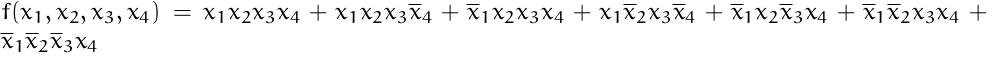
\includegraphics[scale=0.3]{ra38a1.png} \\\\
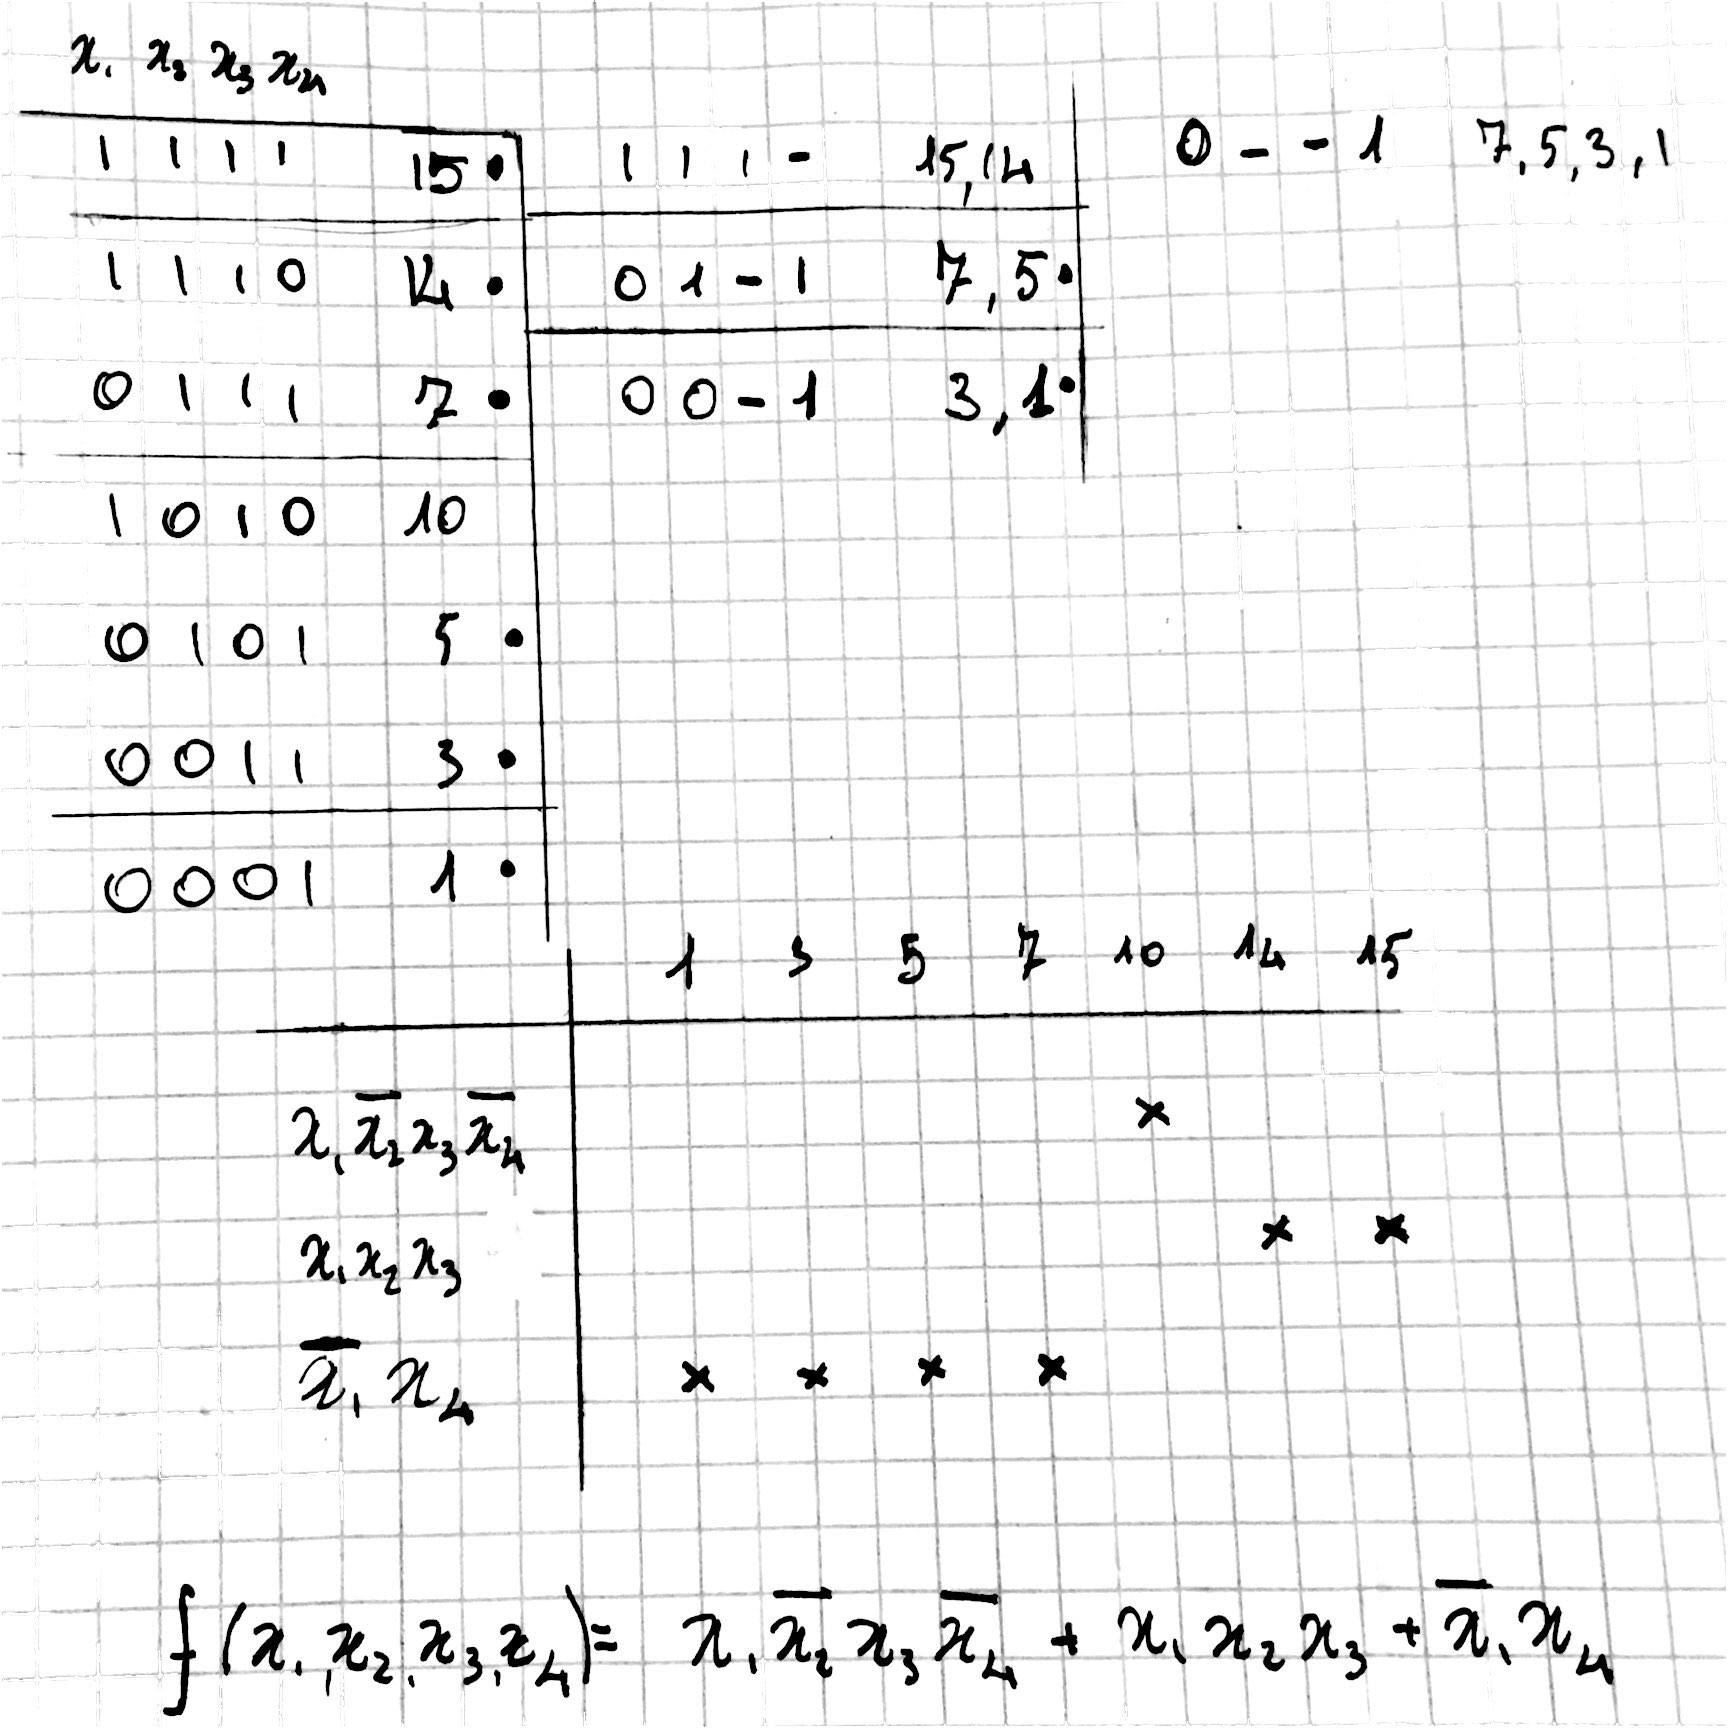
\includegraphics[scale=0.13]{ra38a2_1.jpg} \\
\subsection{b}
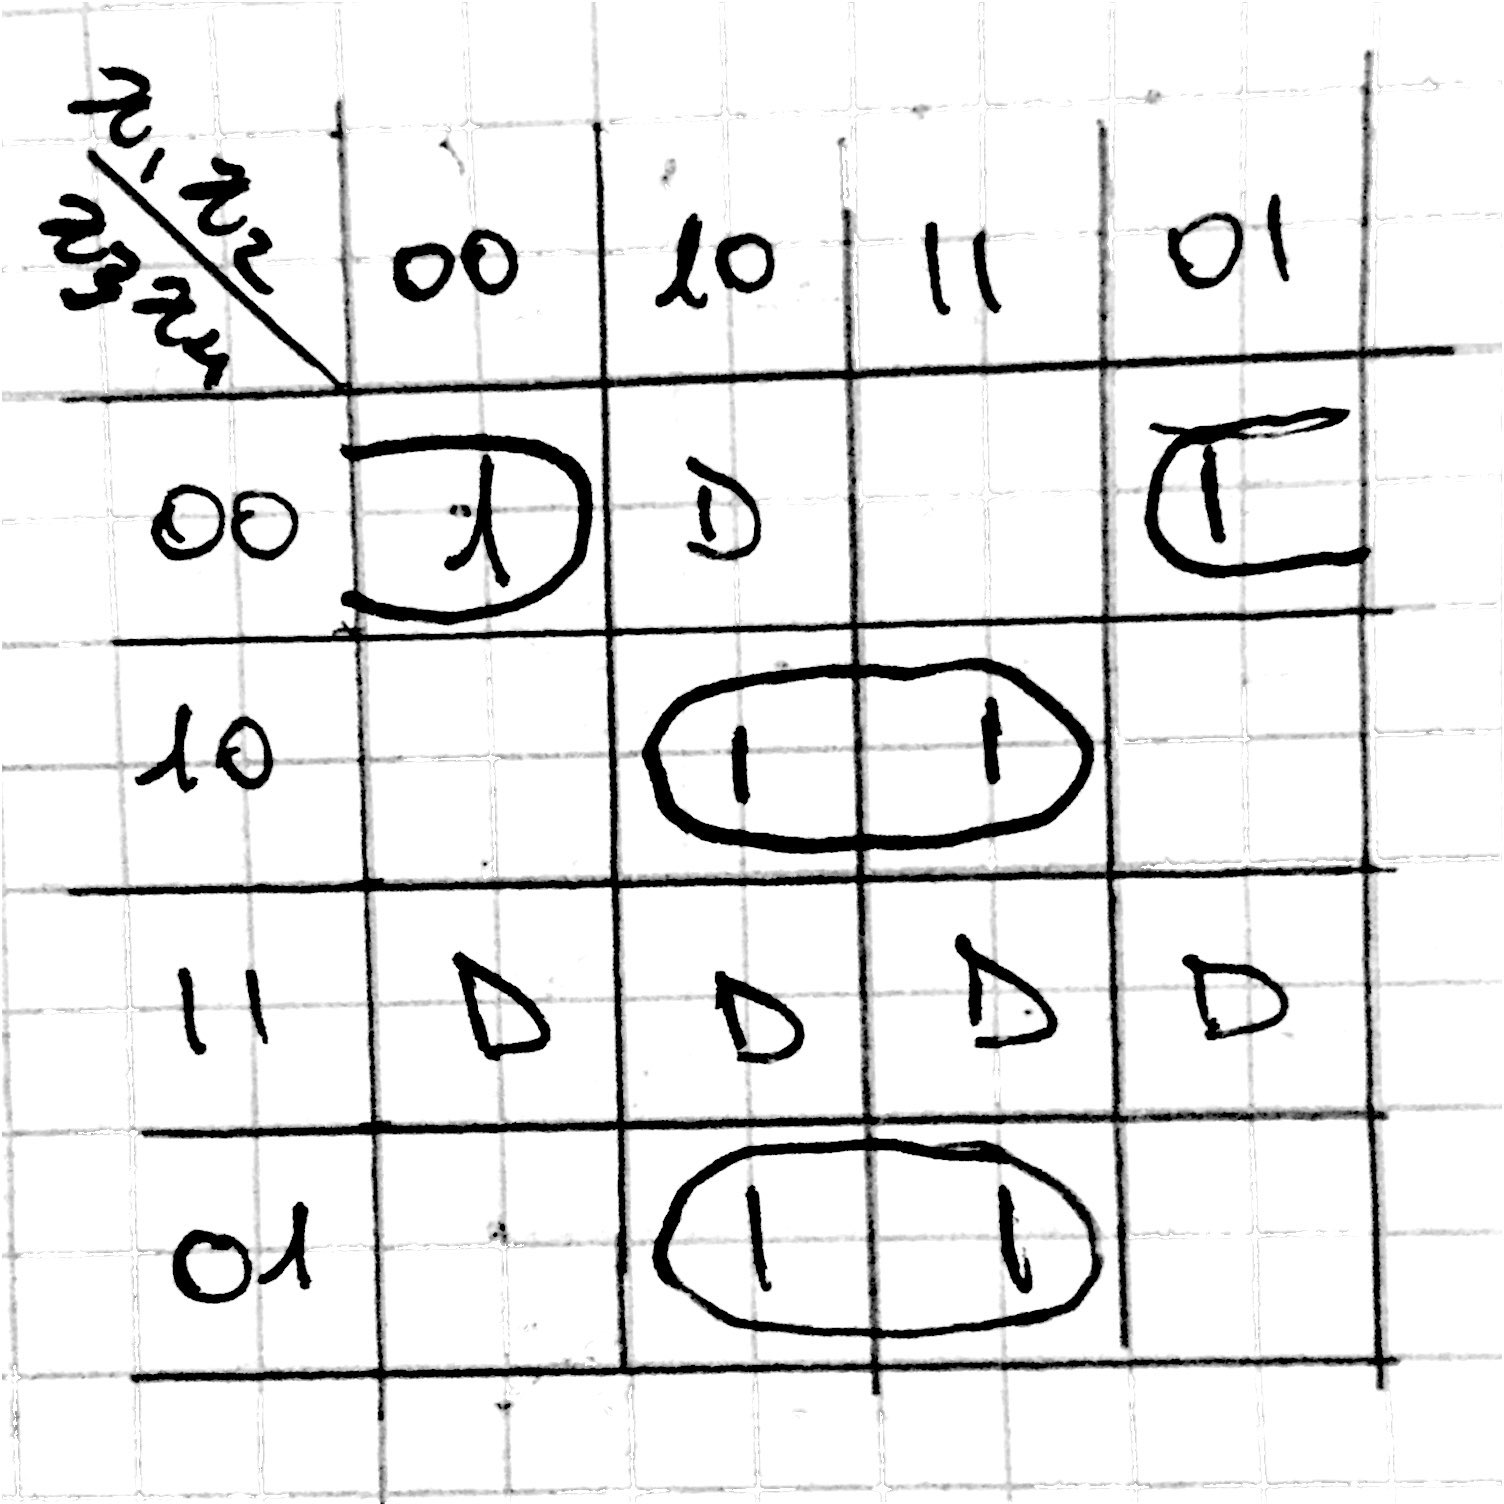
\includegraphics[scale=0.13]{ra38b_1.jpg}\\
$$
	f(x_1,x_2,x_3,x_4)=\overline{x_1}\;\overline{x_3}\;\overline{x_4}+x_1x_3\overline{x_4}+x_1\overline{x_3}x_4
$$
\subsection{c}
Das Verfahren von Karnaugh wird für mehrere inputs schnell unübersichtlich, dagegen bleibt das Quine McQuinley verfahren auch für boolsche Funktionen mit mehreren variablen übersichtlich und erlaubt eine schnelle Vereinfachung.
Zusätlich eignet sich das McQuinley Verfahren mehr an die Automation.

\section{Aufgabe 38}
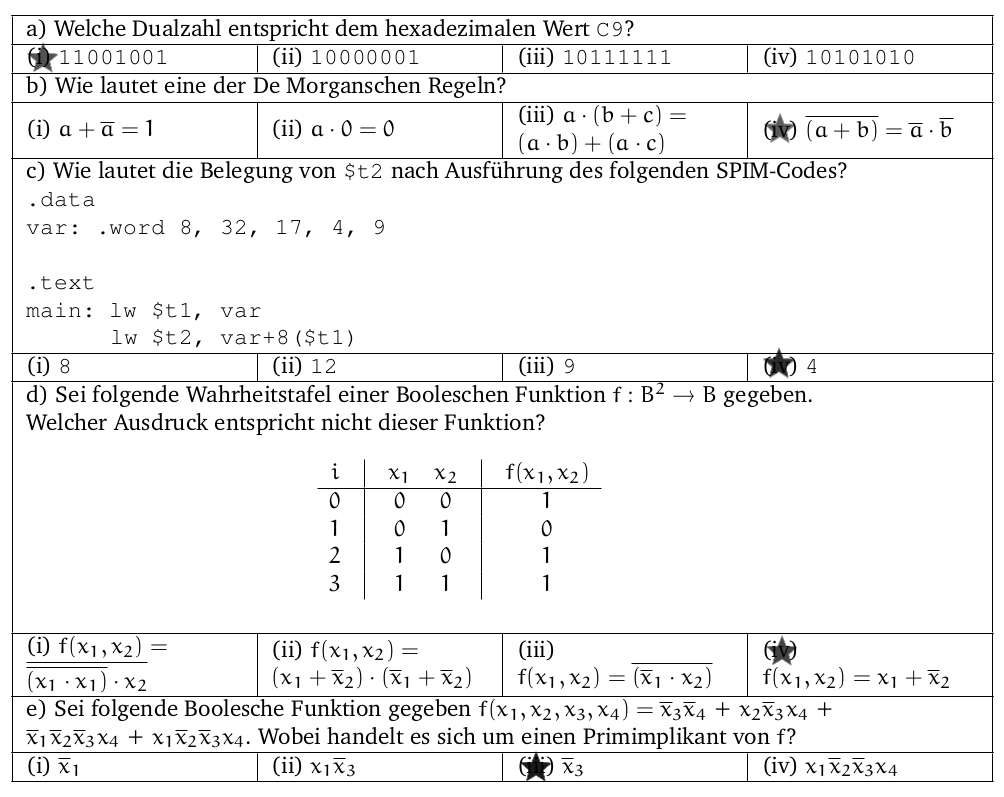
\includegraphics[scale=0.4]{RA39.png}

\end{document}